\label{sec:voterflow}

\begin{figure*}
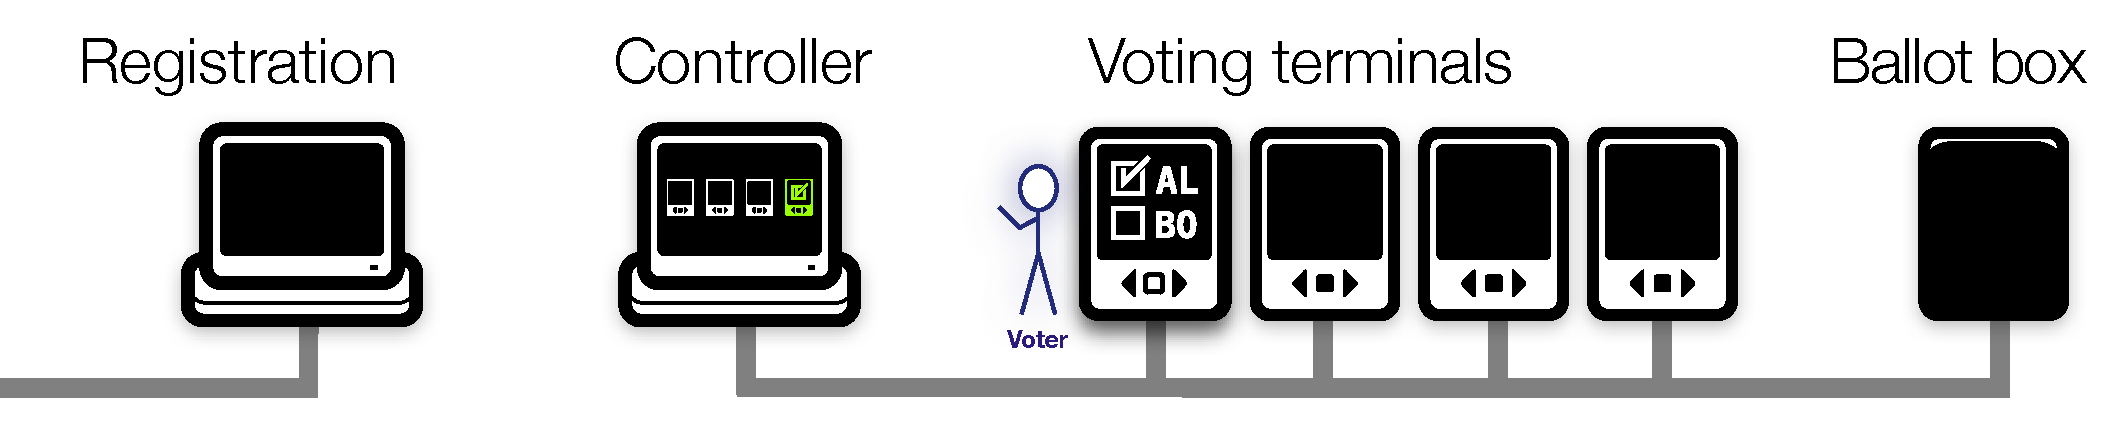
\includegraphics[width=5.5in]{system-layout}
% \caption{The design of the \projname system. Green objects are computers, white objects are paper records, and other objects are shaded in gray. Arrows display the flow of information; green for digital information, black for paper, and dashed lines indicate that the flow is contingent on voter choice.\label{fig:design}.}
\caption{The design of the \projname system. The voter registration
  system (left) is connected to the Internet but not to the internal
  LAN. Voters, move left to right. First, the voter's registration
  is validated, and a thermal printout indicates the proper ballot
  style. This moves to the controller, which scans it and issues the
  voter a PIN, again printed on thermal
  paper. The voter proceeds to any open voting terminal, enters the
  PIN, and is given the proper ballot style. The ballot summary is
  printed, and deposited into the ballot box
  (right). \label{fig:design}}

\end{figure*}

Figure~\ref{fig:design} shows how \projname works from the perspective
of a voter. 
The \projname voting system bears a resemblance to the Hart InterCivic eSlate system and to VoteBox~\cite{sandler08votebox}, in that the voting machines are networked together, 
simplifying the movement of data. 
Like eSlate, our design contains a networked group of voting machines that share a common judge's station with a computer like Hart InterCivic's ``Judge Booth Controller'' (JBC) that manages everything. 

\begin{enumerate}
\item {\em Registration (pollbook).}
The first step for the voter is to check-in with a poll worker. This
is where voter registration is verified and the voter's precinct is
identified so that the appropriate ballot style can be generated. 
The registration system, via cellular modem, notifies a centralized
database of the voter's change in status, to eliminate any risk of
double-voting.

The registration system will
use a thermal label printer to generate a sticker with the
voter's name and precinct indicated (the precinct also indicated with
a 1-D barcode). This sticker goes into a poll book which
the voter signs, providing a backup to the online database.
The barcode can also be read by an off-the-shelf scanner connected to
the controller. This represents the only data flow from the outside
world into the internal voting network, and helps avoid data
entry errors that might come from human transcription. 
Nothing on this sticker is secret nor is anything unique to the
voter. 
Consequently, the flow of this information does not compromise
the voter's privacy, so long as the voter is not the only voter
with the same precinct code to vote at that polling location.

Provisional voters will be indicated with a suitable prefix to their
precinct code, allowing the voting system to suitably distinguish
their ballots from regular ones. (Provisional votes are cast by voters
who, for whatever reason, do not appear in the voter registration
database, and believe this to be in error. They are only tabulated
after the voter's registration status is verified, typically not until
at least a few days after the end of voting.)

\item {\em Controller.}
The controller scans the barcode on the sticker to identify 
the voter's precinct and ballot style. 
The controller then prints a 5-digit code,
unique for the remainder of the election in this polling
place. Holding this printout, the voter can then approach any open
voting terminal, enter the code, and be presented with the correct
ballot style. 
(There will probably need to be a special alternative for ADA
compliance as not all voters can see or handle paper. One possible
solution is that a poll worker could enter the relevant code, then
depart before the voter begins voting.)

There are only ever a small number of 5-digit codes active at any one
time, reducing the odds of a voter successfully guessing an active
code and casting multiple ballots.
We note that there will be no record binding the 5-digit code to the
voter, helping ensure voter anonymity. We also note that these codes
reduce the attack surface, relative to other voting systems that use
smartcards or other active electronic devices to initialize a voting
machine for each voter.

\item {\em Voting terminals.}
 The voter makes selections on the GUI (for sighted voters)
 or auditory UI (for non-sighted voters).
 There is a review screen (or the auditory equivalent)
 so that the voter can confirm all selections before producing a paper record.

\item {\em Print.} When the voter has finished making selections,
  the voting terminal prints two (possibly joined) items:
  (1)~a paper ballot which includes a human-readable summary of the voter's selections
  and a random (non-sequential) serial number, and
  (2)~a paper a take-home receipt that identifies the voting terminal used, the
  time of the vote, and a short (16-20 character) hash code that
  serves as a commitment to the vote but does not reveal its contents.
  The voting terminal also sends data about the vote and receipt
  to the judge's station. (See Section~\ref{sec:crypto} for the exact
  cryptographic design.)


 
  % \COP{Proposal of a variant. There ciphertexts to print are too long
    % when using a homomorphic tallying + we do not want any
    % recognizable link between paper ballots and paper receipts:
% 
% \item {\em Print.} When the voter has finished making selections, she
  % tells the UI to print a paper record of their selections. This
  % cryptographically commits the choices and sends their encrypted
  % ballot to the judge's station as well as printing a paper record, which includes
  % not only a human-readable summary of the voter's selections but a
  % unique serial number (as a bar code or something similar) and a
  % human-readable crypto receipt (essentially a ballot ID number).  }

\item {\em Review printed record.}
The voter may then review the printed record to confirm the indicated
selections. 
There will be at least one offline station available that can 
scan the paper record and read it back to the 
voter for those who cannot visually read the paper record.

\item {\em Option: Cast or challenge/spoil.}
After reviewing the ballot, the voter has a choice: Cast the ballot or spoil it.
 A voter might spoil the ballot because of an error (or change of heart)
 or because the voter wishes to challenge the voting terminal, demanding it to show
 that the voter's selections were correctly recorded and committed to.\footnote{%
 This follows the cryptographic verification process introduced by Benaloh
 in \cite{benaloh06simple} and \cite{benaloh07evt}.
 }
 The two procedures are described below. 
 Note also that there is a special procedure for provisional ballots.

 Regardless, the voter may keep the take-home paper receipt.
 We note that most thermal printers include a cutting device that leaves a
 small paper connection between the two sides of the cut.
 It is therefore a simple matter for the voting terminal to print a single
 sheet that the voter can easily separate into the ballot summary and the
 take-home receipt.
 We also note that ``privacy sleeves'' (i.e., simple paper folders) can protect the privacy of these printed ballots as voters carry them from the voting machine either to the ballot box
 to be cast, or to the judge's station to be spoiled.

\begin{enumerate}
\item  {\em Ballot box: cast ballot.}
A voter who wishes to cast the ballot takes the paper ballot summary to the ballot box.
% The voter optionally removes the receipt and drops it into the box, where the bar code on the record is scanned.
The ballot box has a simple scanner that can read the serial number from the ballot
(the serial number might also be represented as a one-dimensional barcode for reliability)
and communicate this to the controller, allowing the controller to keep a record of which ballots have found their way to the ballot box, and thus, which ballots should be tabulated. 
{\em An electronic ballot record is not considered complete and should not be
 included in the tally unless and until its corresponding paper ballot summary has
 been deposited in the balot box.}

\item {\em Spoil ballot.}
If the paper record is to be spoiled, the voter returns to a poll worker.
% The record will be placed in a special sleeve so that the poll worker cannot see the selections.
The ballot serial number is scanned so that the controller can record
that the ballot is to be spoiled. 
This informs the controller that the corresponding encrypted ballot 
record should not be included in contest results.
Instead, it should be decrypted and published as such after the election is over.
The original printed paper ballot thus corresponds to a {\em commitment\/} 
by the voting machine, before it ever ``knew'' it might be challenged.
 If the voting machine cannot produce a suitable proof that the ballot 
 encryption matches the plaintext,
 then it has been caught cheating.
 Voters who don't care about verification can simply restart the process.
 For voters who may feel uncomfortable with this process,
 as it might reveal their intent to a poll worker,
 we note that voters could deliberately spoil ballots that misstate their true intent. 
 We note that dedicated election monitors could be allowed to use voting machines, 
 producing printed ballots that they would be forbidden from placing in the ballot box, 
 but which would be spoiled and then the corresponding ciphertext would be decrypted. 
 In effect, election monitors can conduct 
 {\em parallel testing in the field\/} on any voting machine at any time during the live election.


\item {\em Provisional ballot.}
In the case of a provisional ballot, the voter does not have the cast
vs.~spoil option, and must return the ballot to a poll worker, who
places it into a distinct provisional ballot box. The voter may retain
the receipt to see if the ballot ends up being counted. Because the
ballot box is connected to the controller over the LAN, it can also
query the controller as to whether the ballot is provisional. In the
event that a voter accidentally puts a provisional ballot into the
ballot box, the scanner can detect this and reject the
pages. (Provisional ballots need to go into dedicated envelopes that
are processed after the voting has ended.)
\end{enumerate}

\item {\em At home (optional): Voter checks crypto.}
The encrypted votes will be posted on a public ``bulletin board''
 (i.e., a web site maintained by the county).
 The voter receipt corresponds to a cryptographic hash of the encrypted vote.
 A voter should be able to easily verify that this vote is present on the bulletin board.
 If a voter spoiled a ballot, that should also be visible on the bulletin board
 together with its decrypted selections.  
 This allows independent observers to
 know which ballots to include in the tally and allows independent verifiers
 to check that all spoiled ballots are correctly decrypted.  
 Individual voters can
 check, without any mathematics,
 that the decryptions of their own spoiled ballots match their expectations.
\end{enumerate}

% << sections 2.2 and 3 should go in here somewhere >>

While this process is more cumbersome than a traditional DRE voting
system, it has a number of advantages. By having the paper elements,
this system not only benefits from sophisticated end-to-end cryptographic
techniques (described in Section~\ref{sec:crypto}), it also can be
audited post-election, by hand, using a risk-limiting audit
(see Section~\ref{sec:audit}). 
Voters also have the confidence that
comes from holding, verifying, and casting a tangible record of their
votes, whether or not they trust the computers.


%%% Local Variables: 
%%% mode: latex
%%% TeX-master: "star"
%%% End: 
